\section{Interpretació de l'enunciat}

En aquest problema tenim una ciutat, passatgers i conductors. Tots els passatgers i conductors
tenen un origen i un destí fixat dins la ciutat on han d'arribar i volem sabre quins conductors
transporten a quins passatgers, sabent la ruta que duen a terme.

Tots els passatgers poden ser recollits per un conductor que el portarà al seu destí,
així doncs un passatger no pot fer el seu trajecte amb més de un conductor.

Hem de tenir amb compte que els conductors tenen una capacitat \emph{C} limitada del vehicle que no pot ser
sobrepassada. Això significa que en un mateix instant no hi pot haver més de \emph{C} passatgers dins un vehicle,
no obstant durant tot el recorregut del conductor pot deixar i recollir diversos passatgers arribant a transportar
més de \emph{C} passatgers\cite{maxCapaDepenentDeRuta}.

\begin{center}[H] \ref{maxCapaDepenentDeRuta}
 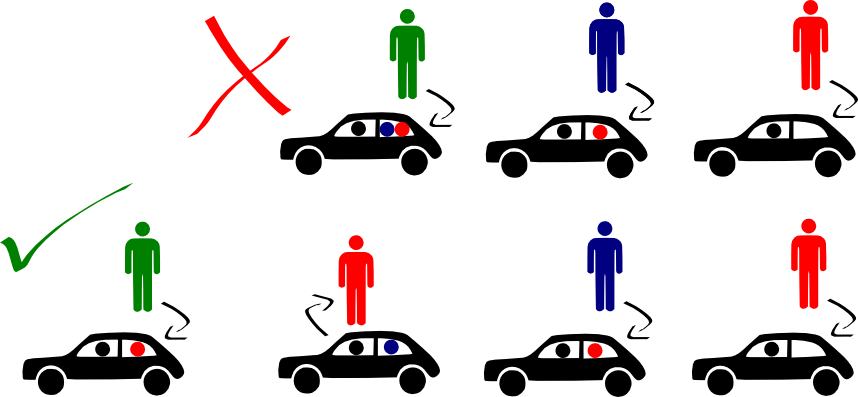
\includegraphics[width=0.6\textwidth]{figures/maxCapaDepenentDeRuta.png}
\end{center}


\emph{Tots} els conductors i passatgers han d'arribar \textbf{a temps} al seu destí. Donat que és
suposa una velocitat \emph{V} constant i que el conductor és l'últim arribar això significa aquest no podrà
superar més d'una determinada distància. En concret es presenta l'escena d'iniciar la ruta a les 7 del mati
i acabar a les 8. Això dona una hora recorregut a velocitat V per el conductor. Si aquesta velocitat es
de 30km/h tenim que un conductor pot recórrer com a molt 30km en la seva ruta. Notem que en l'àmbit
d'aquest problema suposam que el cost temporal de pujar o baixar un passatger és despreciable.

Un conductor pot passar a ser passatger. En tal cas es comportarà com un passatger més. Dit cas
dependrà de la valoració que es faci d'eliminar un conductor o de si comparteix ruta amb un altre
conductor amb espai lliure i que per tant així es minimitza la distància recorreguda.

Donat aquest escenari tenim dos criteris de minimització.
Per una banda volem minimitzar \textbf{la distància total recorreguda} per tots els conductors i per l'altra
a més de minimitzar la distància també volem minimitzar el \texttt{número de conductors}.

Hem de tenir amb compte que dins el primer en certa mesura també s'inclou la minimització de conductors
ja que el còmput de distància es fa per número de conductors i en cas d'haver dos conductors compartint
ruta el fet d'eliminar-ne un resta la distància de la seva ruta minimitzant el còmput total.

En quan al segon criteri s'ha de preveure que número de conductors i kilòmetres són dues unitats de 
mesura diferents que han de donar lloc a una única valoració per tant s'haurà d'establir una manera 
de combinar-les o cercar-hi alguna relació.

\section{Paràmetres}

El número de persones total ve determinat per el paràmetre $N$, de les quals $M$ no són conductors,
son passatgers, així doncs el numero de conductors es $N-P$. 

La ciutat és defineix com una matriu de 10x10 Km on cada illeta es de 100x100 m, així doncs
la ciutat és una matriu de 100x100 illetes.

La distància \emph{D} entre punts (\emph{o}rigen i \emph{d}estí) de la ciutat ve determinada per la funció:
$$ D(o,d) = |o_x - d_x| + |o_y - d_y| $$

Hem de tenir amb compte que la ciutat al ser una matriu per anar d'un punt A a un punt B hi ha múltiples
rutes amb la mateixa distància. Cosa que pot suposar un avantatge ja que així els únics paràmetres
d'una ruta son el punt d'origen, el destí i la distància.
